\chapter{Grundläggande radiokunskap}

\section{Radiovågor}

Radiovågor har fascinerat människan sedan de upptäcktes. De gör det möjligt att kommunicera över stora avstånd och med relativt enkla medel. Till en början var det mycket enkla kommunikationer och det kallades för trådlös telegrafi. Så småningom insåg man att man kunde modulera en bärvåg och överföra tal och musik. Så föddes bl.a. kommunikationsradion med vilken två eller flera människor kan utbyta information och den mer enkelriktade rundradion som sänder ut musik och nyheter än i dag.

Radiovågor i sig är elektromagnetiska till sin natur. Detta betyder att de har en elektrisk komponent och en magnetisk komponent. Båda behövs för att det skall bli en radiovåg. Denna våg skapas i antennen när radion sänder genom att man låter en växelström snabbt gå genom antennen. En ström som går i en ledare genererar ett magnetfält rund denna ledare och för att få ström att flyta behövs en elektromotorisk kraft.

\begin{figure}[h]
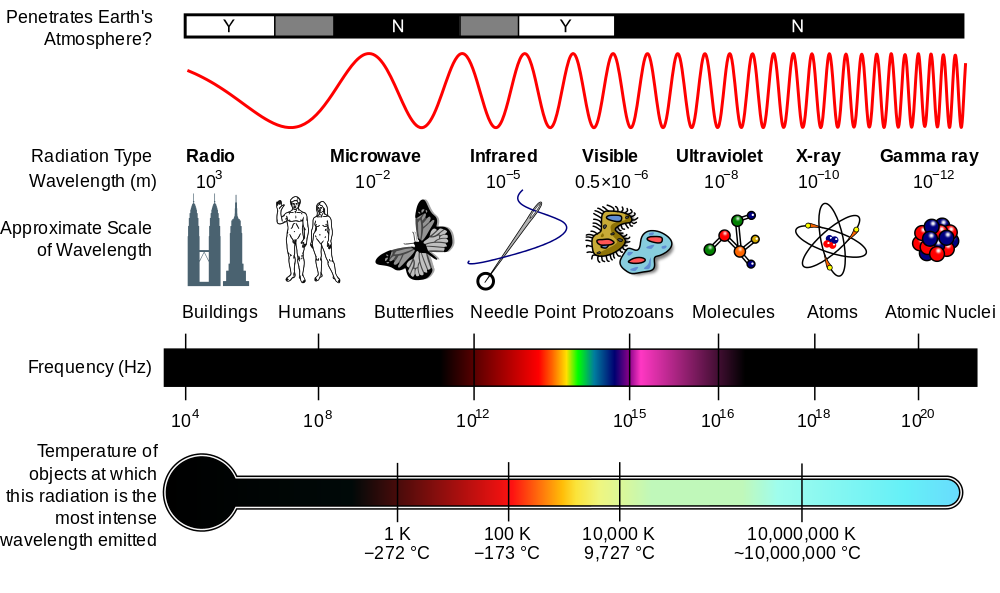
\includegraphics[width=\textwidth]{img/em-spektrum}
\caption{Illustration av elektromagnetiskt spektrum.Källa: \href{https://commons.wikimedia.org/wiki/File:EM_Spectrum_Properties_edit.svg}{Wikipedia}}
\end{figure}

Radiovågen är en sorts elektromagnetisk strålning. En del människor är rädda för strålning men man skall komma ihåg att det finns två sorters elektromagnetisk strålning, så kallad joniserande strålning och icke-joniserande strålning. Om en elektromagnetisk våg är joniserande eller inte bestäms enbart av dess frekvens och för att bli joniserande måste frekvensen vara mycket hög, högre än synligt ljus vilket radiovågor inte är. Radiovågor är alltså icke-joniserande och skall därför inte blandas ihop med radioaktiv strålning.

En radiovåg kan orsaka uppvärmning, det är ju så till exempel mikrovågsugnar arbetar, med tillräcklig effekt på radiosignalen kan den orsaka uppvärmning av vävnader. Med de effekter som vanliga handapparater har, upp till några watt är det ingen fara. Större stationer som amatörradiostationer kan ha flera hundra till tusentals watt och måste hanteras därefter för att man inte skall orsaka problem.

Radiofrekventa vågor (RF) kan också orsaka brännskador redan från någon enstaka watt om man till exempel tar i änden på vissa antenntyper eller håller i en kontakt och sänder samtidigt. Så länge som sändaren inte aktiveras är det dock ingen fara men tänk på att inte sända om ni måste justera en antenn, särskilt gäller detta hemmabyggda antenner.

När man talar om radiovågor talar man framför allt om två storheter. Det ena är frekvensen och det andra är effekten. Ibland talar man ocskå om våglängden men den är egentligen samma sak som frekvensen.

\subsection{Frekvens och våglängd}

En radiovågs frekvens beskriver hur många svängningar per sekund som en radiovåg gör. En sändare alstrar en växelström precis som den växelström vi har i ett vägguttag så har den en frekvens. Strömmen i vägguttaget har en frekvens om 50 Hz vilket betyder att den når sitt största värde 50 ggr per sekund och även sitt lägsta värde 50 ggr per sekund. 

En radiosändare arbetar med mycket högre frekvenser. Från kHz (kilohertz = 1\,000 Hz) och MHz (megahertz = 1\,000\,000 Hz). För oss ligger de mest praktiska frekvenserna i området från ca 1--400 MHz ungefär.

Våglängden beskriver hur långt det är mellan två toppar i svängningen på växelströmmen. Den kan härledas från frekvensen om man vet utbredningshastigheten hos radiovågen och det vet vi, den är ljusets hastighet, ca 300 000 km/s.

Då kan vi skriva följande formel för att översätta mellan våglängd och frekvens:

\begin{equation}
f = \frac{300}{\lambda}
\end{equation}

\begin{equation}
\lambda = \frac{300}{f}
\end{equation}

Här betecknar $f$ frekvensen i MHz och $\lambda$ (lambda) våglängden i meter. 

\begin{table}[!h]
	\begin{tabular}{llrr}
		Frekvensband         & Beteckning &     Våglängd &      Frekvens \\ \hline
		Långvåg              & LV         &     1--10 km &   300--30 kHz \\
		Mellanvåg            & MV         &  100--1000 m & 3000--300 kHz \\
		Kortvåg              & KV         &    10--100 m &     3--30 MHz \\
		Ultrakortvåg         & UKV/VHF    &      1--10 m &   30--300 MHz \\
		Ultrahög frekvens    & UHF        & 100--1000 mm & 300--3000 MHz \\
		Superhög frekvens    & SHF        &  100-1000 mm &     3--30 GHz \\
		Extremt hög frekvens & EHF        &    10-100 mm &   30--300 GHz
	\end{tabular}
	\caption{Frekvenser och våglängder vanligaste banden}
	\label{tab:frekvens-vaglangd}
\end{table}

Tabellen \ref{tab:frekvens-vaglangd} är de generiska benämningar på frekvensbanden som internationella teleunionen (ITU) har fastslagit. Det finns traditionellt andra benämningar också som vi inte kommer gå in på i detalj men rundradiobanden för lång- mellan- och kortvåg följer inte detta slaviskt och för amatörradion brukar 160 m bandet (1\,800--2\,000 kHz) räknas som kortvåg fast det i strikt mening är mellanvåg eller gränsvåg som området mellan 1--3 MHz kallas i marina sammanhang.

\subsection{Polarisation}

Polarisationen hos en radiovåg beskriver hur den elektriska komponenten hos vågen utbreder sig. Den magnetiska komponenten är alltid vinkelrät mot den elektriska. Fälten kallas normalt för E-fält (elektriskt) och B-fält (magnetiskt). Grekiska bokstaven lambda ($\lambda$) betecknar våglängden hos signalen.

Först en bild som visar hur fälten från en antenn kan se ut:

\begin{figure}[h]
	\centering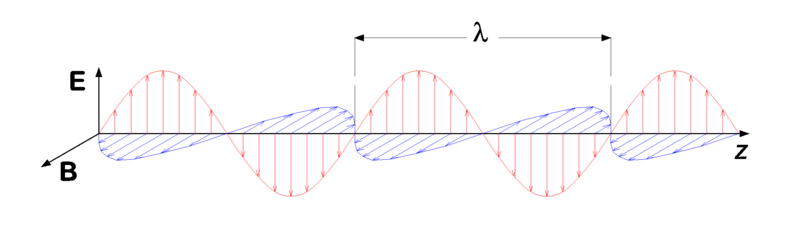
\includegraphics[width=\textwidth]{img/em-wave}
	\caption{E- och B-fältet vertikal polarisation}
\end{figure}

På bilden är E-fältet vertikalt polariserat. De vanligaste antennerna för handhållen och bilburen radio är normalt vertikalt polariserade. För längre kontakter och för trådantenner av dipoltyp är det vanligare med horisontell polarisation. Riktantenner som exempelvis Yagi-Uda (vanliga TV-antenner är ofta av denna typ) kan relativt enkelt ändras i polarisation, man monterar den så att ''pinnarna'' ligger i det plan för den polarisation man önskar.

\begin{figure}[h]
	\centering
	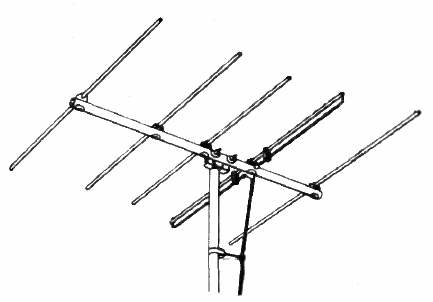
\includegraphics[width=.4\textwidth]{img/yagi-uda}	
	\caption{Yagi-Uda antenn}
\end{figure}

En av de viktigaste sakerna att tänka på när det gäller polarisation är att sändarens och mottagarens antenner skall ha samma polarisation. Om de inte har det kommer man att förlora mycket signalstyrka. Praktiska prov visar att om sändarens och mottagarens antenner är av samma typ, de befinner sig på ett avstånd om ca 10 $\lambda$ från varandra så förlorar man drygt 20 dB om de har olika polarisation. Det är mycket, det innebär endast 1\% av energin når mottagaren mot om de har rätt polarisation!

Polarisationen kan ibland påverkas av terrängen och omgivningen. Exempelvis när en radiovåg reflekteras mot en huskropp kan den komma ut med en annan polarisation än den gick in med. Denna typ av vridningar i polarisationen kan orsaka en ganska kraftig \textit{fädning} av signalen. Fädning innebär att signalstyrkan varierar upp och ned kraftigt, det finns både snabb och långsam fädning och när en sändare och mottagare rör sig relativt varandra hör man ofta ett \textit{flutter} på signalen som ibland kallas \textit{mobilflutter} som mestadels beror på snabb fädning.

För kortvåg och andra frekvenser som nyttjar utbredning i \textit{jonosfären} i luftens översta lager så kan polarisationen komma ned väldigt olika mot hur den sändes. Därför nyttjar man ofta särskilda antenner konstruerade för att ta mot signaler som kommer in brant från jonosfären för att motverka detta.

För VHF och UHF räcker det bra med att tänka på att polarisationen skall vara den samma på sändaren och mottagaren.

\subsection{Impedans}

Impedansen är något som man normalt behöver gå igenom en del växelströmslära för att förstå ordentligt. Det skall vi inte göra här utan vi konstaterar att det finns olika impedanser för matarledningar.

Den vanligaste matarledningen är koaxialkabeln. Den består av en innerledare som är omsluten av en skärmad återledare. Skärmen är normalt jordad vid radion och detta kallas för en obalanserad matarledning. 

I praktiken finns det två sorter i dag, 75 $\Omega$ (Ohm) impedans som används till exempel för kabel-TV och liknande. Alla radiosystem i dag använder sig av 50 $\Omega$ system. Det går i nödfall att använda sig av 75 $\Omega$ kabel men det rekommenderas inte då den inte väl matchar radion eller antennen. Dessutom skiljer det ofta något på kontakter vilket medför att exempelvis BNC-kontakter kan råka skadas om man sätter en 75 ohms-kontakt i en 50-ohms chassiedon vilket senare kan leda till glapp och problem.

Om det finns för stora impedansskillnader på matarledningen jämfört med antennen eller radion får vi problem med att effekten inte hamnar i antennen på rätt sätt utan vi får reflektion av effekten vilket värmer upp slutsteget i onödan. Gamla apparater kan gå sönder av det, moderna har som regel skydd för det och apparater med låg effekt (någon watt) brukar heller inte gå sönder av det. Det är av samma anledning som man \textit{aldrig skall sända med öppen antennkontakt}. I det fallet blir reflektionen total och all utgående effekt reflekteras tillbaka till sändaren. 

Hur stor reflektion man har mäts antingen sin VSWR eller i \textit{return loss}. Den föra betyder \textit{voltage standing wave relation} och den andra mäts i dB som beskriver hur mycket effekt under den framåtgående som reflekteras. Genom att mäta stående vågförhållandet (framåtgående respektive reflekterad effekt) hos en antenn kan man få en indikation på hur antennen fungerar. Dock är det inte alltid så att alla fel kan upptäckas. En matarledning med hög förlust gör att stående vågen också ser bättre ut nere vid radion men antennen fungerar inte bättre för det. 

För att analysera stående vågen hos en antenn behövs i regel en antennanalysator eller ett instrument som kan mäta både den framåtgående och reflekterade effekten. Ett sådant instrument är ganska nödvändigt om man skall bygga egna antenner. Det finns enkla modeller att få tag i för ungefär en näve hundralappar och uppåt på Ebay och liknande ställen. En del säljs som byggsatser man själv bygger samman, det brukar kräva att man är någorlunda händig med en lödpenna och montera komponenter på mönsterkort, en del finns färdiga och kostar också därefter. Se till att skaffa en mätare som klarar alla frekvensbanden som du tänkt använda.

\section{Effekt och räckvidd}

En radios effekt mäts oftast i watt i lekmannamässiga sammanhang medan i professionella sammanhang så använder man decibel. Decibel är dock inget effektmått i sig, det beskriver egentligen skillnaden mellan två effekter men när man talar om en radios effekt används ibland enheten dBm som betyder antal decibel från 1 milliwatt (mW).

\subsection{Watt och dBm}

Om en sändare har 1 mW (milliwatt) uteffekt sägs den ha 0 dBm. Om den har 1 W uteffekt är det 30 dBm och om den har 10 W uteffekt är det 40 dBm.

Varför vi gärna använder dBm har att göra med att det blir lättare att beräkna hur långt en radiosignal kommer om vi har dessa siffror. 

Att räkna om från watt till dBm görs med följande ekvation:

\begin{equation}
P_{\mathrm{dBm}}=10\cdot\log(P_{\mathrm{W}}\cdot 1000)
\end{equation}

Omvänt kan vi också räkna om det enligt:

\begin{equation}
P_{\mathrm{W}}=\frac{10^{\mathrm{P_{dBm}}/10}}{1000}
\end{equation}

Där $P$ betecknar effekten i watt eller dBm och faktorn 1000 kommer med för det är milliwatt vi egentligen räknar om till och från dBm. Se tabellerna \ref{tab:effekt-dbm} och \ref{tab:oversattning-w-dBm} för mer information och översättning mellan de båda enheterna.

\begin{table}[!h]
	\centering
 	\begin{tabular}{rr|rr}
	      Watt & dBm &   Watt & dBm \\ \hline
	      1 nW & -60 &  10 mW &  10 \\
	     10 nW & -50 & 100 mw &  20 \\
	    100 nW & -40 &    1 W &  30 \\
	  1 $\mu$W & -30 &   10 W &  40 \\
	 10 $\mu$W & -20 &  100 W &  50 \\
	100 $\mu$W & -10 &   1 kW &  60 \\
	      1 mW &   0 &  10 kW &  70
	\end{tabular}
	\caption{Effekt i W och dBm från små till stora effekter}
	\label{tab:effekt-dbm}
\end{table}

\todo{dB och faktorer i tabellform}

\subsubsection{Räkna decibel i huvudet}

För att underlätta förståelsen och att räkna med decibel så finns det ett antal trick man kan komma ihål. Varje 10 dB är en tiodubbling. Varje -10 dB är en tiondel. I dBm utgår vi från 1 mW. Eftersom 1 W är 1000 gånger 1 mW innebär det att det är tre 10-dubblingar och det blir därför $10+10+10=30$ dBm.

3 dB är en fördubbling och -3 dB är en halvering. För att berälna hur många watt 43 dBm är så kan vi tänka oss följande: 1 W är 30 dBm. 10 dB till betyder gånger 10 alltså är det 10 W. 3 dB på det är en fördubbling. Alltså är 43 dBm lika med 20 W. 

Vi kan också minnas att 1 dB är ungefär 20\% mer och -1 dB är ungefär 20\% mindre. Nu har vi verktygen att stega i steg om 10 / 10 dBm, i steg om 2 / 3 dB och i steg om 1.2 / 1 dB.

Beräkna hur många dBm en radio på 5 W har. Vi vet att 1 W = 30 dBm och om vi fördubblar till 2 W blir det 33 dBm. Fördubblar vi igen blir det 4 W och 36 dBm. 5 W är ungefär 20\% mer än 4 W så vi lägger till 1 dB och får 37 dBm vilket är mycket nära det exakta svaret.

\subsubsection{Decibel och faktorer}

Omvandlingen mellan decibel och faktorer och tvärt om är kanske överkurs men bra ändå att känna till. Det man kan läsa ut ur denna tabell är att 7 dB upp innebär en ökning av effekt med 5,01 gånger.

Likaså kan man läsa att om man delar effekten på tre vägar får varje väg 4,72 dB lägre effekt.

\begin{table}[H]
	\centering
	\begin{tabular}{rr|rr}
		dB & Faktor & Faktor &    dB \\ \hline
		 0 &   1,00 &        &       \\
		 1 &   1,26 &      1 &  0,00 \\
		 2 &   1,58 &      2 &  3,01 \\
		 3 &   2,00 &      3 &  4,72 \\
		 4 &   2,51 &      4 &  6,02 \\
		 5 &   3,16 &      5 &  6,99 \\
		 6 &   3,98 &      6 &  7,78 \\
		 7 &   5,01 &      7 &  8,45 \\
		 8 &   6,31 &      8 &  9,03 \\
		 9 &   7,94 &      9 &  9,54 \\
		10 &  10,00 &     10 & 10,00
	\end{tabular}
\end{table}

\subsection{Utbredningen av en radiovåg}

En radiovåg utbreder sig med ljusets hastighet egentligen i alla riktningar. Nu är de flesta antenner så konstruerade att de kraftigt undertrycker vissa riktningar och premierar andra. En handapparat med sin antennpinne på radion är i det närmaste rundstrålande men strålar inte uppåt och nedåt särskilt mycket. Normalt har man heller inte så stor användning för effekten åt dessa håll varför det verkar vettigt.

Radiovågens effektdensitet kan ses som ytan hos en expanderande sfär. Den avtar därmed kvadratiskt med avståndet från sändaren och därmed är den effekt en mottagare kan ta mot omvänt proportionerlig mot kvadraten på avståndet.

Låter det krångligt? Egentligen är det inte så märkligt, man kan säga att den mottagna effekten blir bara en fjärdedel om jag dubblar avståndet. Om jag tripplar avståndet blir den en niondel och så vidare.

I decibel säger vi att effekten sjunker med 6 dB varje gång vi fördubblar motståndet. Detta gör att om vi känner avståndet mellan sändare och mottagare kan vi beräkna den förlust som vi har på grund av utbredningen. Detta kallas normalt för \textit{sträckdämpningen} och kan relativt enkelt beräknas.

\subsection{Sträckdämpning}

Men det finns även andra faktorer som spelar in och som påverkar radiovågens styrka. Exempelvis blir antenner kortare med minskad våglängd (eller ökad frekvens) och det gör att den area som kan ta upp radiovågen också minskar. Så detta behöver vi ha med i formeln och det visar sig att den är också omvänt proportionell mot kvadraten på antennens längd.

Slutligen så är det ju så att terrängen har betydelse. Om vi bara räknar med ovanstående parametrar så får vi något som kallas för \textit{free space path loss} alltså sträckdämpning i fria rymden. Eftersom vi befinner oss på marken med allt vad det innebär av terräng och blockeringar så måste vi även räkna med detta.

Att få det exakt är mycket svårt och kräver simuleringsmodeller som är utanför det vi kommer gå igenom här. Däremot kan vi göra kvalificerade gissningar om vi känner våra radioapparaters effekter, mottagarens känsligheter, antennernas egenskaper och terrängen mellan.

\subsection{Mottagarens känslighet}

En mottagares känslighet är avgörande för hur bra man hörs. En mpottagare som lyssnar där det inte finns någon signal och har en öppen brusspärr hör egentligen det som brukar kallas för termiska bruset.

Detta uppkommer på atomnivå när elektriskt laddade partiklar som elektroner utbyter fotoner med varandra. Det finns ett sätt att beräkna detta brus och det är temperaturberoende. Genom att räkna på detta i t.ex. rumstemperatur (20 grader C eller 300 K ungefär) får vi fram en förväntad bruseffekt.

En radio behöver sedan en signal som är starkare än det bruset för att kunna demodulera signalen. För FM-radio av walkie-talkie typ så säger man att det behövs minimum 12 dB starkare signal än bruset.

Vi kan beräkna bruset för en 25 kHz FM-kanal till ca -130 dBm. Om vi sedan lägger på 12 dB till detta samt en brusfaktor på 6 dB för mottagarens egenbrus så får vi -112 dBm. Detta är den känslighet en radio normalt har för FM-mottagning givet inga andra störningar. Sedan finns det ju mer eller mindre bra mottagare också, en del kan vara ganska mycket sämre som t.ex. de flesta enkla PMR446-apparater.

På PR-bandet får man även räkna med en ganska stor mängd elektriska störningar och det kan även vara så i stadsmiljö på VHF och ibland även uppe på UHF-bandet.

Vi sammanfattar med att i bästa fall är känsligheten hos en vanlig FM-kom\-ra\-di\-o\-mot\-ta\-ga\-re ca \textbf{-112 dBm}. Detta skall vi lägga på minnet.

\subsection{Antennens egenskaper och kroppsdämpning}

Antennen på radion har stor betydelse. De flesta handapparater har en enkel antennkonstruktion som kallas kvartsvågsantenn. Den är alltså ungefär 1/4 så lång som våglängden. 

Många apparater använder samma antenn för flera frekvensband, den kan då vara mer eller mindre väl anpassad för dessa och det finns olika sätt tillverkarna gör för att få antennen bra på flera band.

\subsubsection{Antennvinst}

I datablad ser man ofta beteckningar på hur bra en antenn är och det finns två sätt att ange den så kallade antennvinsten: dBd och dBi.

Det första begreppet dBd talar om hur mycket bättre (eller sämre) antennen är jämförd med en väl avstämd dipolantenn. Det andra sättet jämför med en teoretisk helt isotrop antenn som inte finns i verkligheten utan bara i tanken och i matematiska modeller. Det går att omvandla mellan dBd och dBi enligt följande:

\begin{equation}
G_{\mathrm{dBi}} = G_{dBd} + 2,15
\end{equation}

\begin{equation}
G_{\mathrm{dBd}} = G_{dBi} - 2,15
\end{equation}

Beteckningen $G$ står för antennvinst (gain) i detta sammanhang. Antennvinsten beror på att antennen inte strålar likvärdigt i alla riktninar. En dipolantenn strålar ungefär som en torus (tänk dig en frityrmunk) och strålar alltså inte ut från ändarna utan det är bredsidan på antennen som strålar mest. Denna \textit{sammantryckning} av strålningsdiagrammet ökar effekten i vissa riktningt.

\subsubsection{Antennens riktverkan ger antennvinsten}

Detta är det som avses med antennvinsten. En del riktantenner kan ha väldigt hög antennvinst, vanliga antenner på walkie-talkies brukar ha några dB. Om en antenn görs lång och med speciella trick kan man trycka ihop strålningsloberna ännu mer och då får man en högre antennvinst.

Dock blir den också mer och mer riktningskänslig och det blir noga med riktning och placering av antennen. Exempel på antenner med hög antennvinst och stor känslighet är till exempel parabolantenner. Exempel på antenner med inte lika hög antennvinst och riktningskänslighet är vanliga tv-antenner.

\subsubsection{Antennvinst i reklamen}

Ett varningens ord också för antenntillverkare i främst Asien som ofta kommer med riktiga glädjesiffror och heller inte skriver ut om det är dBd eller dBi. Strunta i dessa siffror, de är inte relevanta. Alla enkla antenner som är baserade på en dipol ligger runt ca 2 dBi i antennvinst. 

Hos en handhållen radio med 1/4-vågsantenn är antennvinsten i praktiken inte mer än någon dB. För en fritt hängande dipol är den 2,15 dBi. De flesta enkla antenner ligger däromkring. Kolinjära eller på annat vis stackade antenner kan komma upp i några dB till i antennvinst.

\subsection{Kroppsdämpning}

När vi står nära en antenn, som vi gör med en handhållen radio, befinner vi oss i antennens strålningsfält. Detta gör att vi påverkar hur antennen fungerar och det är i princip aldrig vi gör den bättre. 

Detta brukar benämnas som kroppsdämpning, \textit{eng. Body Loss}, och gör att antennen fungerar sämre än den annars skulle ha gjort. En frihängande antenn däremot exempelvis en dipolantenn eller någon av dess varianter som en \textit{Slim Jim} kan man räkna utan kroppsdämpning.

För antenner som matas med koaxialkabel så räknar man i stället för kroppsdämpning med förlusten i matarkabeln. 

Kroppsdämpningen är oftast i storleksordningen 1-3 dB och dras från antennvinsten när man skall beräkna utbredningen. Det gör att vi i de flesta fall kan betrakta handhållen radio som 0 dBi i den bästa riktningen.

\subsection{Penetrationsförlust}

En radio som används inomhus, i ett fordon av något slag, bakom hinder av olika typer och så vidare drabbas av en så kallad penetrationsförlust. Denna beror på att radiovågen hindras mer när den skall tränga igenom en glasruta (mest reflektion) eller hitta ut genom en bil eller liknande. 

Penetrationsförlusten kan uppskattas till ca 15 dB i en bil för dessa band, kansk 20 dB för moderna bilar med metallfilm i rutorna och upp emot 30 dB från en modern plåtklädd tågvagn och så vidare.

Om man befinner sig på sådana ställen kan en yttre antenn vara till stor hjälp. De flesta radioapparater har en kontakt om man skruvar av den ordinarie antennen på vilken man kan ansluta en antennledning som exempelvis går till en magnetfot med yttre antenn ovanpå biltaket.

Magnetfot är fint för det fungerar i många sammanhang och kan enkelt flyttas från fordon till fordon utan att det kräver någon installation. Det fungerar också hjälpligt på ett balkongräcke eller fönsterbleck från en lägenhet eller hus.

\todo{Bild på magnetfot}

\subsection{Terrängens påverkan}

Terrängen påverkar landmobil radio något oerhört. Vi kan med lätthet säga att den påverkan är större än några av de andra faktorerna som vi hittills har gått igenom. När man pratar i en handburen radio får man vara beredd på att göra små förflyttningar fram och tillbaka för att hitta en plats där det fungerar bra.

Man skall inte ha radion i bältet och använda lös mikrofon. Även om detta kan verka coolt och fint sjunker verkningsgraden rejält. Dels ligger radions antenn mot kroppen i det närmaste och den skärmar. En annan sak som händer är att antennen på en handhållen radio behöver en motpol. När du håller i radion är du motpolen och förbättrar verkningsgraden, när den hänger i bältet blir detta sämre.

\subsubsection{Terräng och val av frekvensband}

I terrängen finns det kullar och berg, klippor, fält och sjöar och andra saker som påverkar utbredningen. Nära vatten kan radiovågen gå mycket bra över vattenytan, i skog och mark med tätt mellan träden och steniga kullar dämpas signalen mycket mer.

Generellt sett utbreder sig VHF bättre i skog och mark och över vatten än UHF gör. Dock är antalet kanaler som vi kan nyttja lagligen begränsade i bandet även om det på senare tid kommit flera frekvenser som är tillåtna att användas.

Här ligger också de så kallade jaktkanalerna på 150 MHz-bandet av samma anledning.

I bebyggelse dämpar husen också liskom i urban miljö de stora husen. Här kan man ibland nyttja att högre frekvenser reflekterar sig bättre mellan hus och glasrutor och man kan därför ha större chans att komma fram på UHF än på VHF

På UHF finner vi de flesta kanalerna på 400 MHz-bandet och att det är väl använta i urban miljö förstår vi då exempelvis bilräddningskåren, väktarbolagen, taxi med flera ofta använder detta band. Det finns också ett större frekvensutrymme för egna kanaler i detta band och för PMR-radio finns det flera olika frekvenser upplåtna.

Som prepper bör UHF vara förstahandsvalet i urban miljö medan VHF kommer till sin rätt ordentligt i glesbygden och framför allt i skogen.

\subsubsection{Terrängfaktorn i utbredningsformeln}

Om vi skall kunna beräkna utbredningen behöver vi kunna hantera terrängen på något sätt, detta gör vi med en terrängfaktor. Terrängfaktorn väljs enligt följande:

\begin{table}[h]
\centering
\begin{tabular}{rl}
	Faktor & Terrängbeskrivning                            \\ \hline
	     0 & Fri rymd, förekommer i det närmaste inte      \\
	     5 & Över sjö, något mindre över saltvatten        \\
	    10 & Flack terräng eller utbredning över vatten    \\
	    15 & Bebyggd glesbygd eller kulligare terräng      \\
	    20 & Tät bebyggelse eller bergig terräng           \\
	    25 & Mycket urban bebyggelse, extremt svår terräng \\
	    30 & Torr stenöken
\end{tabular}
\caption{Terrängfaktorn}
\end{table}

\subsection{Beräkning av räckvidden}

Nu har vi tillräckligt med information för att kunna beräkna vilken signalnivå som en mottagare placerad på ett visst avstånd från en sändare i en given terräng, på ett känt frekvensband och med de antennegenskaper vi känner göra en hygglig beräkning på om det fungerar eller inte.

Vi börjar med formeln för utbredning:

\begin{equation}
L_P = 20\cdot\log(f)+(20+K)\cdot\log(d)+32,45
\end{equation}

Här finner vi att $L_P$ är sträckdäpningen (\textit{Path Loss}) $f$ är frekvensen i MHz och $d$ är avståndet i km. Faktorn 32,45 är utbredningen som en area på en sfär och omräknat till decibel och justerat för kilometer. Om man föredrar att räkna i mil ändrar man faktorn till +52,45 i stället och om man föredrar i meter blir den -27,55.

Faktorn $K$ terrängfaktorn som vi normalt väljer meöölan 5--15 ungefär beroende på hur tuff terrängen är för radiovågen.

Vi beräknar sedan egenskaperna hos sändaren och mottagaren:

\subsubsection{Sändaren}

För sändaren är det den effektivt isotropt utstrålade effekten vi vill ha (EIRP) och den beräknar vi genom följande:

\begin{equation}
P_{\mathrm{EIRP}}=P_{\mathrm{TX}} + G_{\mathrm{dBi}} - L_{\mathrm{body}}
\end{equation}

Om vi så antar en radio på 5 W vilket är 37 dBm och en antennvinst på 2 dB samt en kroppsförlust på 2 dB så får vi följande:

\begin{equation}
P_{\mathrm{EIRP}}=37 + 2 - 2 = 37
\end{equation}

Utstrålad effekt är alltså 37 dBm EIRP.

\subsubsection{Mottagaren}

Vi kan konstatera att mottagarens känslighet är ca -112 dBm. Vi gör en liknande beräkning här och antennvinsten förbättrar känsligheten (ger lägre värde) och kroppsdämpningen försämrar den (ger högre värde). 

Eftersom kroppsdämpningen och antennvinsten verkar ta ungefär ut varandra kan vi använda -112 dBm direkt.

Tänk på att detta gäller endast FM-mottagning och vid en bandbredd på ca 25 kHz (normal komradio-FM).

\subsubsection{Totala sträckdämpningen}

Den totala maximala sträckdämpningen kan nu beräknas som skillnaden av dessa två tal:

\begin{equation}
L_{\mathrm{max}} = P_{\mathrm{TX}} - S_{\mathrm{RX}}
\end{equation}

I exemplet ovan får vi:

\begin{equation}
L_{\mathrm{max}} = 37 - (-112) = 149
\end{equation}

Nu vet vi att vi kan inte överskrida detta tal i sträckdämpning för då kommer inte radioföbindelsen fungera. Nu kan vi sätta i det där i den totala formeln och kontrollera om vi kan höra varandra på 5 km håll i medelsvår terräng på frekvensen 156,000 MHz.

Vi väljer terrängfaktorn 20 för denna beräkning.

\subsubsection{Slutför beräkningen}

\begin{equation}
L_P=20\cdot\log(156)+(20+20)\cdot\log(5)+32,45 = 43,9 + 28,0 + 32,45 = 104,35
\end{equation}

Om inga andra störningar finns så bör förbindelsen kunna fungera. Observera att detta gäller endast när både sändare och mottagare befinner sig på \textit{relativt höga och fria positioner mot omgivningen}. 

Är man nere i terränglådan kommer möjliga förbindelsesträckan att förkortas avsevärt.

\subsubsection{Fri sikt fungerande kommunikation}

Ibland hör man uttrycket att VHF och UHF går lika långt som ögat ser. Det stämmer ganska bra för handhållet att man kommer till den synliga horisonen men relativt ofta kommer man även längre.

\subsection{Använda effekt med omdöme}

När man sänder bör man försöka begränsa effekten så mycket som det går utan att den tänkta mottagaren får problem att läsa det som sägs i radion. 

De allra flesta radioapparater har minst två effektsteg, hög och låg, inte sällan är hög ca 4--5 W och låg 0,5--2 W. I de allra flesta lägen brukar de flesta allid ha radion inställt på högeffektsläget för att nå så långt som möjligt.

I ett läge där radiokommunikation ersätter annan fjärrkommunikation är det inte alltid önskvärt att göra på det sättet, kanske av många olika skäl.

Anledningarna till att begränsa sin effekt är flera. De mest uppenbara är förstås att genom begränsning i uteffekten uppnår man följande:

\begin{itemize}
	\item En högre effekt gör det möjligt för andra längre bort att avslyssna sändningen
	\item En högre effekt tär mer på batteriet i sändaren
	\item En högre effekt riskerar störa andra som använder samma radiofrekvens
	\item Automatiska pejlar bestämmer din position inom någon sekund från att du börjar sända om minst 2 stationer hör dig
\end{itemize}

Man skall alltså använda effekter med omdöme för att inte i onödan röja sig eller göra slut på batterierna.

En radioapparat i mottagning drar också en del ström. De flesta moderna handapparater klarar ungefär en dags passning innan batteriet börjar att tryta. Om batteriet är gammalt eller inte fullt laddat blir tiden förstås kortare.

Vid sändning underlättar det om man sänder sitt meddelande i ett svep, mottagaren kan sedan bekräfta att det tagits mot ordentligt varpå man sedan är klar. Att föra långa konversationer använder onödigt mycket batteriström.

Mer om detta i kapitel  \ref{kap:radiotrafik} om radiotrafik.

\section{Bandbredd}

\todo{Förklara bandbredd för AM, FM, SSB}

\section{Egenskaper hos olika band}

De band vi talar mest om här är medelhöga delen på VHF, 136--174 MHz och lägre delen av UHF ungefärligen 400-470 MHz. UHF-bandet har förstås ganska olika egenskaper när man kommer upp på de höga delarna som 1-3 GHz men där finns inte så många frekvenser som är vettiga för PMR.

Värt att notera är att idag ligger alla mobiltelefonifrekvenser i UHF-bandet från ca 800--2700 MHz.

\subsection{VHF/UKV}

UKV är en äldre beteckning på bandet som ofta avsåg rundradiobandet (88--108 MHz) men ibland betecknade hela det som i dag benämns VHF.

VHF betecknar frekvenser mellan 30-300 MHz. VHF-bandet där komradio förekommer är ett intressant band som om man planerar sin användning kan nå miltals med, ända till horisonten, om man har bra antenner och fri sikt. 

Effekten är inte lika viktig, faktum är att 5 W (37 dBm) räcker väldigt bra, om man skall göra en rejäl skillnad behöver man öka effekten ungefär tiofallt till 50 W (47 dBm) för att det skall bli en avgjord skillnad. 

Störningsnivåerna på VHF kan ibland vara katastrofala, särskilt i urbana miljöer. I glesbygd och ute i skog och mark är det ofta mycket bättre men ibland är det störningar även här. 

Vädret kan påverka signalen också. Vissa typer av väder där ett varmare luftlager ligger ovanför ett kallare lager vid marken, så kallad \textit{inversion} kan göra så att signalen studsar mellan marken och detta luftlager och plötsligt nå mycket långt. Detta kan inträffa på våren och på hösten mestadels.

På natten går VHF något längre än på dagtid men det är inte som med till exempel kortvåg där skillnaden kan vara enormt stor mellan dag och natt.

I terrängen går VHF bäst eftersom del lite längre våglängden mindre hindras av terrängen och växtligheten. Däremot kan man behöva flytta lite på sig fram och tillbaka för rätt position, våglängden är ungefär 2 meter och genom att flytta sig någon halvmeter kan det göra stor skillnad.

\subsection{UHF}

UHF-bandet omfattar frekvenser från 300 MHz till 3 GHz. UHF-bandet där komradio förekommer är ett mycket bra band för kommunikation så långt som ögat når. Detta band påverkas mindre av väderförhållanden än VHF men i gengäld har det också något kortare utbredning (om man jämför samma typ av antenner). Samtidigt är det också på grund av den kortare våglängden (ca 70 cm) enklare att bygga antenner med högre antennvinst vilket lätt kompenserar för utbredningsförlusterna.

Störningsnivåerna på UHF är ofta bättre från elektriska saker men däremot är störningsnivåerna från andra radiosystem på närliggande frekvenser ofta ett långt större problem. Många kommunikationsnät nyttjar frekvenser runt 400 MHz och det innebär att kommer man nära dessa basstationssändare kan man lätt bli störd av dessa.

UHF har vissa fördelar i urban miljö, det reflekterar sig lättare exempelvis runt husväggar och mot glasrutor, har något bättre penetration i vissa byggmaterial och så vidare.

Därför upplever många det som att bandet \textit{går bättre} i stan medan man på landsbygden hellre använder VHF.

Det är också i UHF-bandet som vi finner de flesta fria PMR-frekvenserna som vi kan använda för att prata på lagligt. Därför är det rekommendabelt att försöka få kontakt på UHF först och VHF kan provas om UHF inte fungerar.

